\subsection{Results}\label{ssec:M2:results}


\subsubsection{Electron fraction} \label{sssec:M2:results:electron_fraction}

\begin{figure}[ht!]
    % 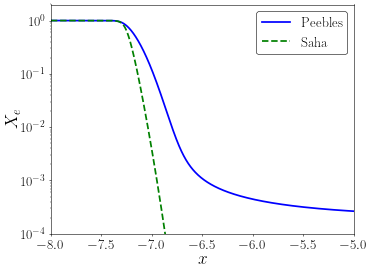
\includegraphics[width=\linewidth]{TEMPcompare_Xe_peebles_saha.png}
    \includefig{compare_Xe_peebles_saha}
    \caption{Free electron fraction computed from the Saha equation only (dashed green curve) and from the Peebles equation (solid blue curve), where the Saha equation was used at early times, until $X_e<0.99$.}
    \label{fig:M2:results:compare_Xe_peebles_saha}
\end{figure}


\begin{figure}[ht!]
    % 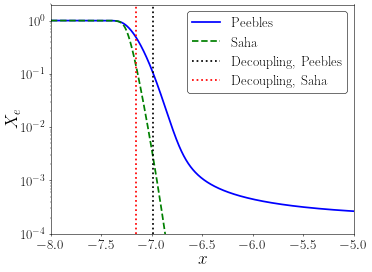
\includegraphics[width=\linewidth]{TEMPdecoupling_compare_Xe_peebles_saha.png}
    \includefig{decoupling_compare_Xe_peebles_saha}
    \caption{Free electron fraction computed from the Saha equation only (dashed green curve) and from the Peebles equation (solid blue curve), where the Saha equation was used at early times, until $X_e<0.99$. The decoupling time, i.e. when $\tau=1$, is shown for both the Saha solution (dotted red curve), and for the Peebles solution (dotted black curve).}
    \label{fig:M2:results:decoupling_compare_Xe_peebles_saha}
\end{figure}

\begin{figure}[ht!]
    % 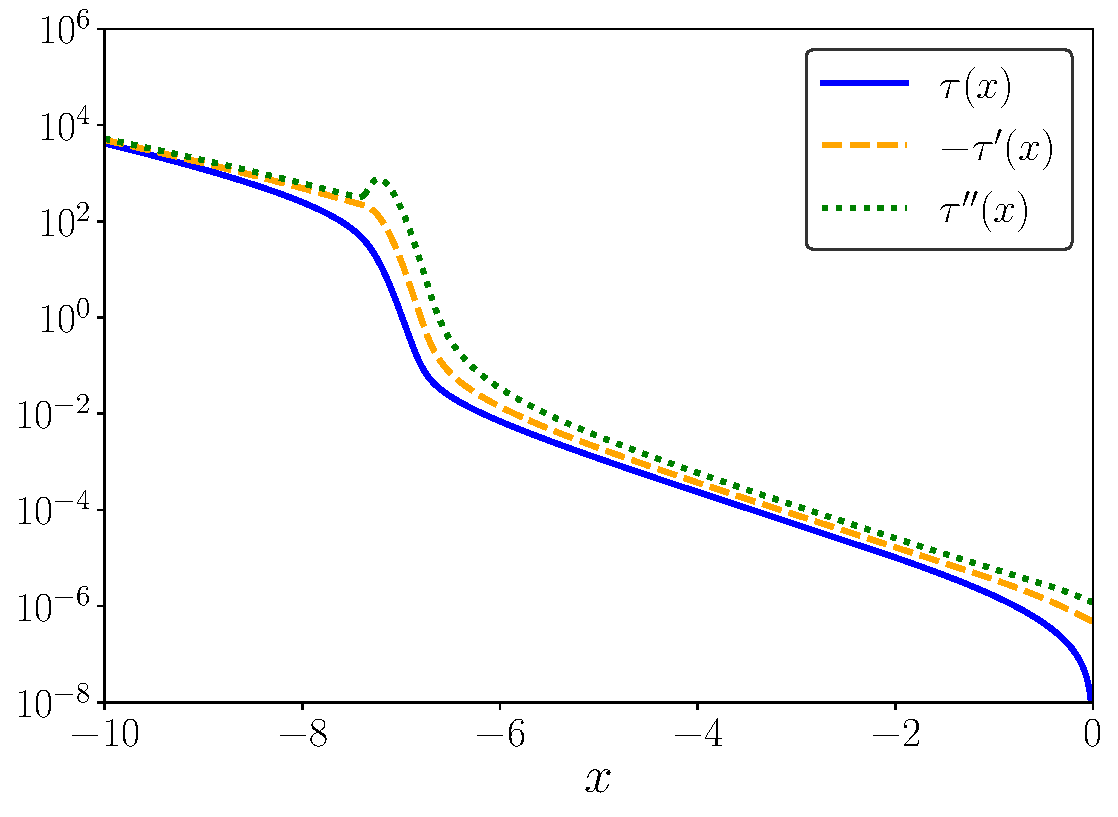
\includegraphics[width=\linewidth]{tau_plot.pdf}
    \includefig{tau_plot}
    \caption{The optical depth, $\tau(x)$ and its two first derivatives with respect to $x$.}
    \label{fig:M2:results:tau_plot}
\end{figure}


\begin{figure}[ht!]
    % 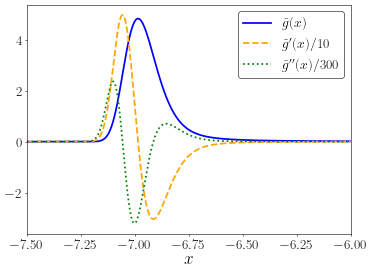
\includegraphics[width=\linewidth]{TEMPg_plot.png}
    \includefig{g_plot}
    \caption{The visibility function, $\gx$ (solid curve), and its derivatives, $\g'(x)/10$ (dashed curve) and $\g''(x)/300$ (dotted curve). The derivatives have been scaled in order to view them all in the same plot.}
    \label{fig:M2:results:g_plot}
\end{figure}

\tablesMilestoneTwo{rec_and_dec_time_table_Peebles.tex}

\tablesMilestoneTwo{rec_and_dec_time_table_Saha.tex}


This is given in table \ref{tab:M2:results:rec_and_dec_time_table_Peebles}